\section{Marco conceptual}

\subsection{Datos ómicos}

Las ciencias ómicas conocidas también como biomedicina o bioinformática, estudian los procesos biológicos a nivel molecular a través de grandes conjuntos de datos con el fin de diagnosticar, prevenir y predecir enfermedades, así como también en terapias y tratamientos personalizados en pacientes (Figura \ref{fig:dat_omic}). El término de “omica” se deriva del griego "óma" que significa masa o conjunto \citep{ravi2016deep,mamoshina2016applications}. La omica es un campo de la biomédica con una gran extensión y esta se divide en diferentes ramas como la genómica, transcriptómica, proteómica, metabolómica, epigenómica, farmacogenómica y metagenómica.

\begin{figure}[h!]
    \centering
    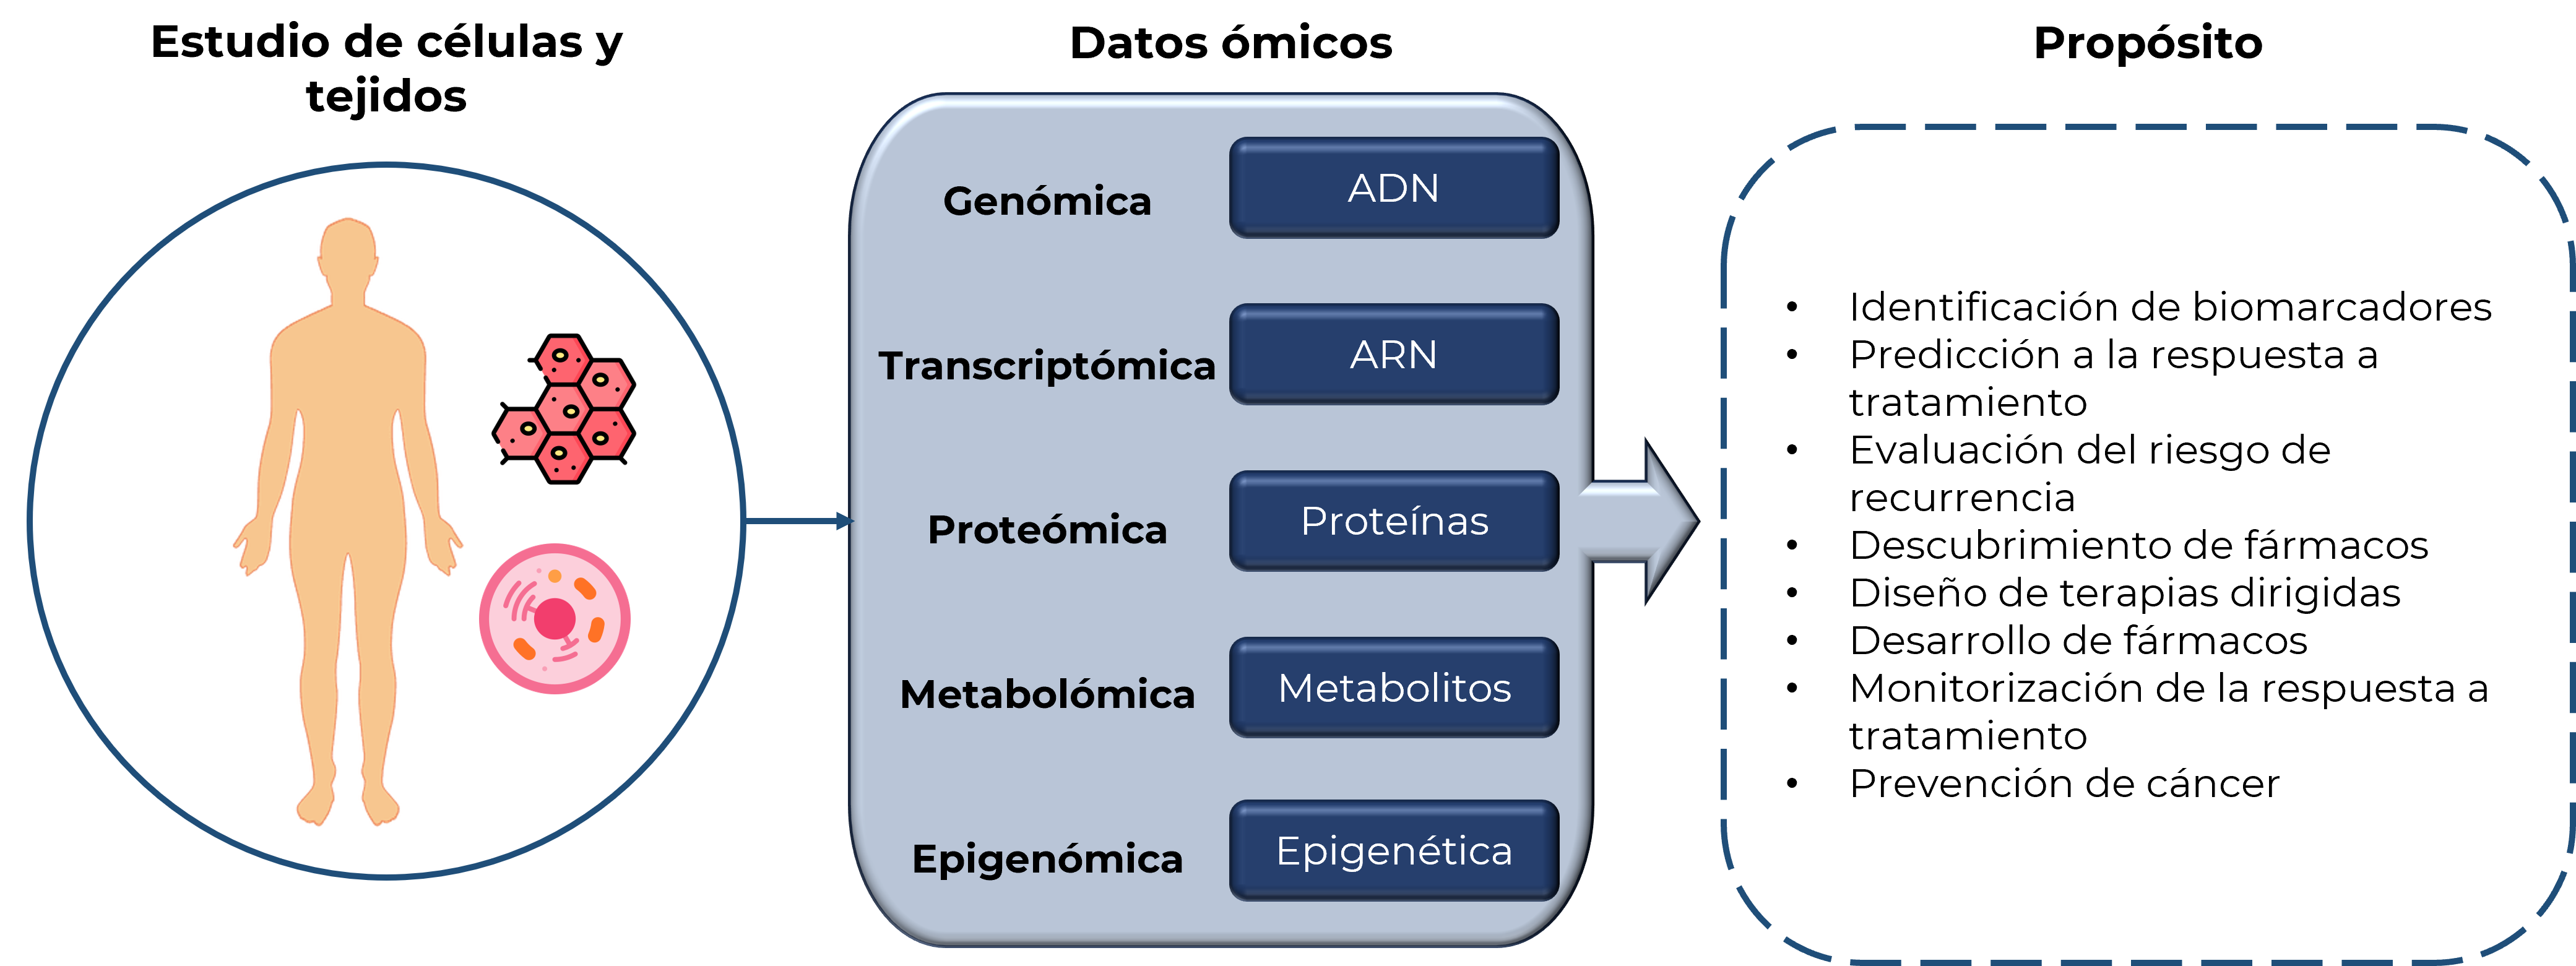
\includegraphics[width=0.9\textwidth]{Imagenes/Datos_omicos.png}
    \caption{Diagrama de la obtención y propósito de los datos ómicos}
    \label{fig:dat_omic}
\end{figure}

\subsection{Tipos de ciencias ómicas}

Las diferentes ramas de la ómica se dirigen a distintos niveles moleculares, habitualmente se estudian de manera independiente a la hora de abordar enfermedades y obtener conocimiento médico y científico, cada una ofrece información importante, pero en conjunto las ciencias permiten obtener relaciones de los niveles moleculares y entender su complejidad biológica (Figura~\ref{fig:tip_omic})

\begin{figure}[h!]
    \centering
    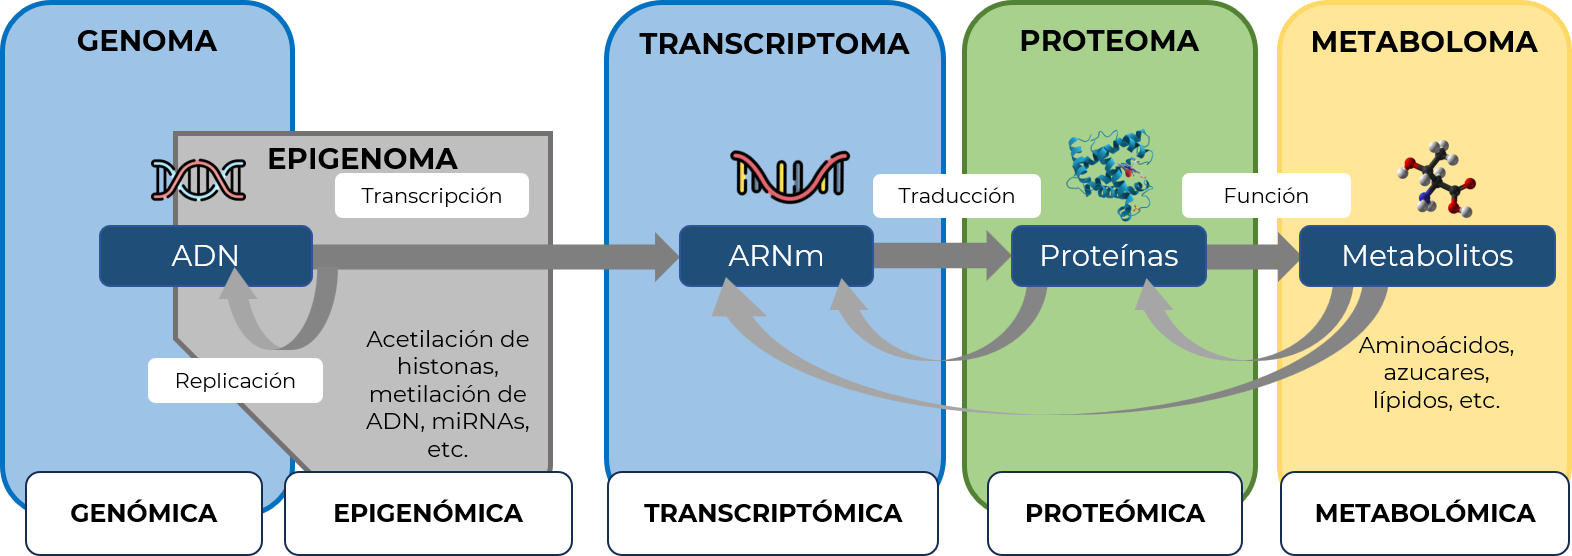
\includegraphics[width=0.9\textwidth]{Imagenes/Tip_omic.png}
    \caption{Clasificación de ciencias ómicas y relación entre ellas}
    \label{fig:tip_omic}
\end{figure}



La genómica es de las primeras ciencias ómicas en reconocerse como tal, esta se encarga del estudio de los genomas, es decir, la totalidad del material genético que tiene un organismo vivo o una partícula viral. El objetivo es identificar alelos genéticos y factores ambientales que contribuyen al desarrollo de enfermedades \citep{institute}.

La transcriptómica estudia el patrón de la expresión genética en un organismo o en células específicas bajo circunstancias concretas, es decir, el conjunto de los ARN mensajeros (ARNm) y no codificantes, a nivel cuantitativo y cualitativo \citep{davis2017missing}.

La epigenómica estudia el conjunto de modificaciones reversibles del ADN o de las proteínas asociadas al ADN (como las histonas) que actúan como elementos funcionales de regulación de la expresión génica de una célula sin alterar la secuencia de su ADN \citep{hasin2017multi}.

La proteómica estudia el conjunto de las proteínas con sus isoformas y modificaciones postraduccionales expresadas en una celular, tejido u órgano concreto en un momento dado, bajo determinadas condiciones y localización específica, dado que las proteínas median las actividades bioquímicas en una célula \citep{van2018precision}.

La metabólica es la ciencia que estudia el conjunto completo de los metabolitos (intermediarios metabólicos, hormonas y metabolitos secundarios) que se encuentran en un momento dado en una célula, tejido u órgano. Entre los metabolitos estudiados se incluyen desde el oxígeno, los aminoácidos esenciales o las vitaminas \citep{zhao2014lipidomics}.

\begin{table}[!h]
    \scriptsize
    \centering
    \caption{Listado de ciencias ómicas establecidas}
    
    \begin{tabular}{
    >{\centering\arraybackslash}m{4cm} 
    >{\centering\arraybackslash}m{9cm}}
\hline 
        \textbf{Ciencia ómica} & 
        \textbf{Área de estudio}
\\      
    \hline \hline 

    Genómica &
    Estudio del conjunto del material genético presente en un organismo.
\\
    \hline
    Transcriptómica &
    Estudio de los perfiles de expresión de los ARN mensajeros, los microARNS y ARN no codificantes.
\\
    \hline
    Epigenómica &
    Estudio de los elementos que controlan la expresión génica sin modificar la secuencia de nucleótidos del ADN.
\\
    \hline
     Proteómica &
     Estudio del set completo de proteínas expresadas en un organismo en un tiempo determinado y particular de cada tipo celular o tisular.
\\
     \hline
     Metabolómica &
     Identificación y cuantificación de productos metabólicos de pequeño tamaño (metabolitos) de un sistema biológico (célula, tejido, fluido biológico u órgano)
\\
     \hline
     Farmacogenómica &
     Estudio de los genes que afectan a la respuesta de una persona a determinados fármacos
\\
     \hline
     Metagenómica &
     Estudio del conjunto de microorganismos de una muestra ambiental para proporcionar información de la diversidad ecológica de un ambiente determinado.
\\
    
\hline
    \end{tabular}
    \label{tab:List_omic}
\end{table}

En la tabla~\ref{tab:List_omic} siguiente se resume la información de las ciencias ómicas establecidas y su definición por área de estudio.



\subsection{Representación de datos ómicos}

En cada ciencia ómica se tiene un tipo distinto de representación de acuerdo al tipo de datos que se extraen, esto es fundamental para el almacenamiento, análisis e interpretación de este tipo de datos, para permitir a los investigadores extraer características biológicas, en la Tabla~\ref{tab:Datos_cod} se muestra la forma en que se representa cada dato:

\begin{table}[!h]
    \scriptsize
    \centering
    \caption{Representación de los datos más frecuentemente utilizados}
    
    \begin{tabular}{
    >{\centering\arraybackslash}m{4cm} 
    >{\centering\arraybackslash}m{9cm}}
\hline 
        \textbf{Tipos de datos} & 
        \textbf{Descripción de la representación} 
\\      
    \hline \hline 

    Genómicos &
    Secuencias de ADN, representadas por cadenas de 4 caracteres.
\\
    \hline
    Transcriptómicos &
    Perfiles de expresión genética, representados por una tabla o matriz numérica.
\\
    \hline
    Epigenómicos &
    Señales registradas en un vector que contiene series temporales o perfiles, representadas en una tabla de valores numéricos.
\\
    \hline
     Proteómicos &
     Secuencias de proteínas, representadas por una cadena de 20 caracteres. Espectrometría de masas, representada por un vector con serie temporal.
\\
     \hline
     Metabolómicos &
     Cálculo de espectro, representado por vector con series temporales.
     Perfiles, representados en una tabla con valores numéricos.
\\
    
\hline
    \end{tabular}
    \label{tab:Datos_cod}
\end{table}

\subsection{Datos ómicos en oncología}

Los datos ómicos en la investigación del cáncer son una herramienta importante, por medio de estos es posible analizar a gran escala las moléculas y las interacciones que existen en las células tumorales. A partir de estos se proporciona una visión global y detallada de los mecanismos moleculares que intervienen en el desarrollo y progresión del cáncer, permitiendo nuevas vías en el diagnóstico, pronostico y tratamiento \citep{olivier2019need}. En siguiente tabla se muestra las principales ciencias ómicas utilizadas en oncología y la información que proporcionan en actividades de diagnóstico, pronóstico y respuesta al tratamiento de la investigación del cáncer.

\begin{table}[!h]
    \scriptsize
    \centering
    \caption{Datos ómicos en oncología}
    
    \begin{tabular}{
    >{\centering\arraybackslash}m{2cm}
    >{\centering\arraybackslash}m{4cm}
    >{\centering\arraybackslash}m{4cm} 
    >{\centering\arraybackslash}m{4cm}}
\hline 
        \textbf{Ciencia ómica} & 
        \textbf{Diagnóstico} & 
        \textbf{Pronóstico} & 
        \textbf{Respuesta al tratamiento}

\\      
    \hline \hline 

    Genómica &
    Diagnóstico de tipo de cáncer y tipos moleculares. &
    Alteraciones genómicas asociadas a un pronóstico bueno o malo. &
    Identificar mutaciones para predicción de la respuesta a terapias dirigidas.
\\
    \hline
    Transcriptómica &
    Análisis de ARNm para identificar subtipos de cáncer (comportamientos clínicos) &
    Patrones de expresión génica para predicción de probabilidad de recurrencia o metástasis. &
    Expresión de genes para predecir la respuesta a quimioterapia o radioterapia.
\\
    \hline
    Proteómica &
    Proteínas presentes en las células tumorales (perfiles proteicos) para el diagnóstico temprano &
    Presencia o ausencia de proteínas que está asociado con un pronóstico bueno o malo &
    Perfiles proteómicos para predecir la respuesta a terapias dirigidas (Eficiencia de fármacos).
\\
    \hline
    Metabolómica &
    Alteraciones metabólicas para diagnóstico temprano &
    Perfiles metabólicos para predicción de progresión de cáncer y respuesta a tratamiento. &
    Alteraciones metabólicas que influyen en la respuesta a quimioterapia y radioterapia.
\\
     \hline
     Epigenómica &
     Alteraciones epigenéticas del ADN para biomarcadores para diagnóstico y clasificación del tipo de cáncer. &
     Patrones de metilación de ADN asociados con un pronóstico bueno o malo. &
     Alteraciones epigenéticas  que influyen en la respuesta a quimioterapia y otros tratamientos.
\\
    \hline
    \end{tabular}
    \label{tab:Omic_onco}
\end{table}

\subsection{Redes neuronales artificiales}
%Fuente: https://doi.org/10.18273/revuin.v19n4-2020001

 Las ANN son un modelo de algoritmo computacional inspirado en las redes biológicas, con el que se establecen relaciones entre las entradas y salidas. Se caracteriza por ser una herramienta que tiene la capacidad para aprender, procesar y generalizar automáticamente datos, utilizadas en tareas de clasificación y regresión \citep{NeuronalNet2014}. En el propósito de clasificación, los datos de entrada son clasificados en distintas clases, y en la regresión, o aproximación de función, se realiza para predecir un parámetro de salida desconocido \citep{NeuronalNet2014}. Es por esto que las ANN cuentan con el potencial en aplicaciones de reconocimiento de patrones y predicción de comportamiento.

 \subsubsection{Componentes de la red neuronal}

 Una neurona artificial se compone de una o múltiples entradas $p$, un peso $w$, un bias o umbral $b$, un sumador $\sum$ y una función de activación $f$, como se puede observar en la Figura~\ref{fig:Neu_Diag}. 

 \begin{figure}[!h]
     \centering
     
\includegraphics[width=0.8\textwidth]
     {Imagenes/Neu_Diag.png}
     \caption{Representación de neuronas artificiales de una entrada y múltiples entradas \citep{NeuronalNet2014}.}
\label{fig:Neu_Diag}
 \end{figure}

 Normalmente, una neurona con múltiples entradas suele no ser suficiente, por lo que las ANN se usan con varias neuronas ubicadas en paralelo formando un “capa”. Las ANN pueden poseer una capa o múltiples como se observa en la Figura~\ref{fig:Net_conjunt}.

  \begin{figure}[!h]
     \centering
     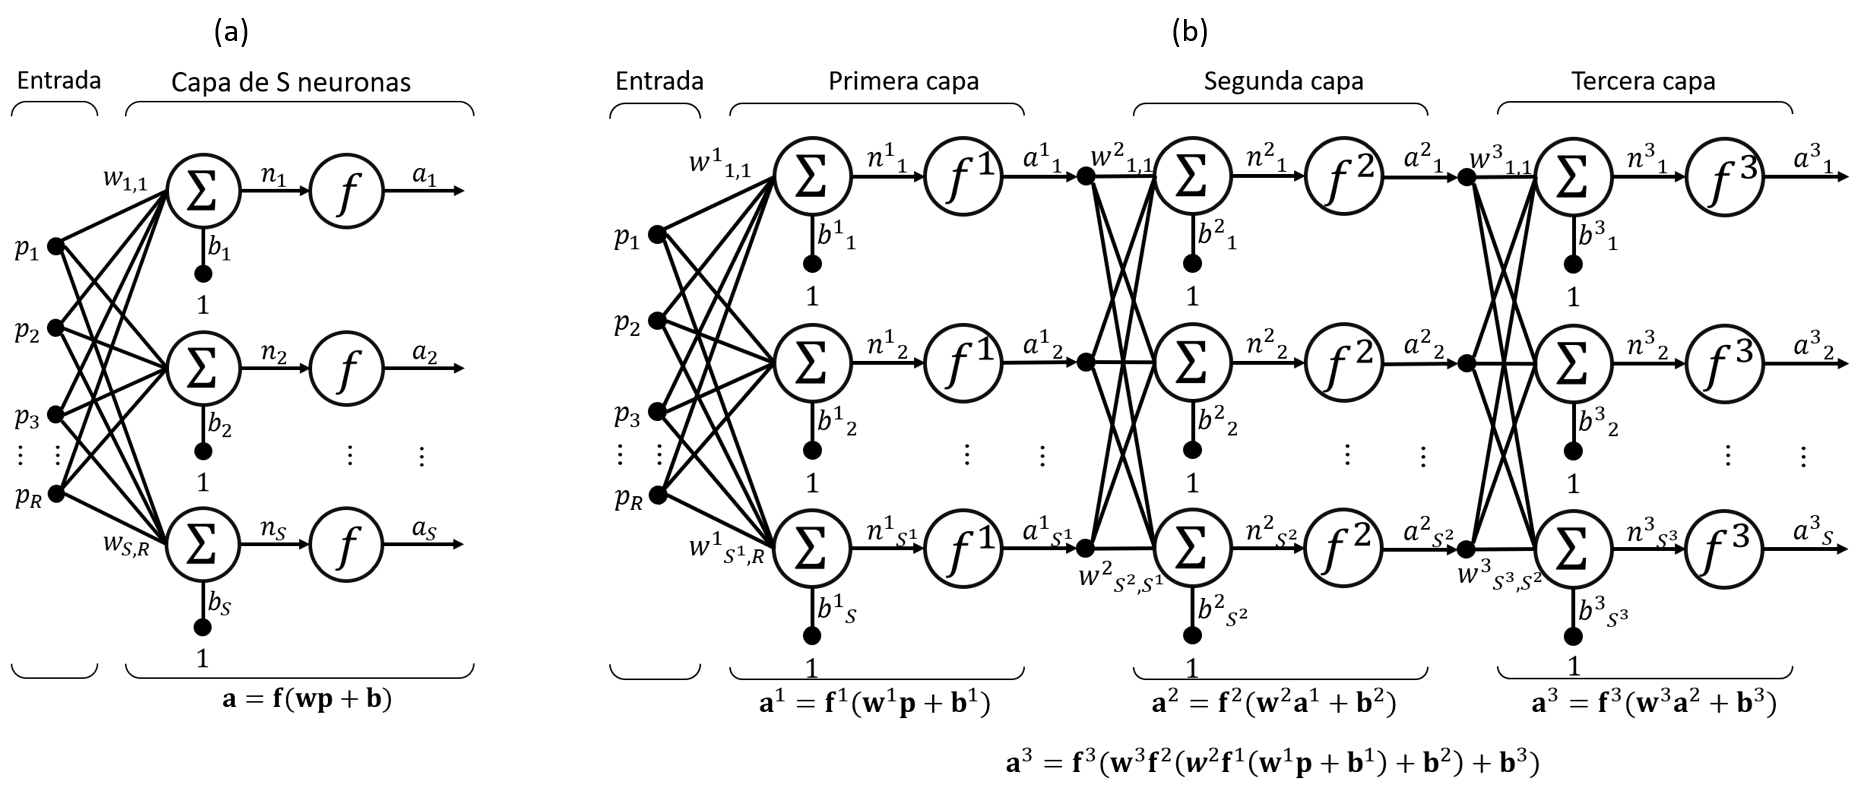
\includegraphics[width=.9\textwidth]{Imagenes/ConjuntoANN.png}
     \caption{Redes neuronales artificiales: (a) de capa oculta y (b) múltiples capas.}
    \label{fig:Net_conjunt}
 \end{figure}


El perceptron es conocido por ser el primer modelo de red neuronal, utilizado en clasificación de patrones a partir de entradas escalares binarias o vectores bipolares \citep{rosenblatt1958perceptron}. El algoritmo de aprendizaje se basa en la regla de Hebb, usando conjunto de datos de entrenamiento  para obtener los pesos de la red a través de iteraciones inicialmente con valores aleatorios.

\subsubsection{Funciones de activación}

Las funciones de activación es una función matemática que determina la salida de una neurona artificial en función de su entrada. Esta función introduce no linealidad en el modelo, lo que permite a las redes neuronales aprender y modelar relaciones complejas entre los datos de entrada y salida \citep{dubey2022activation}. Las funciones desempeñan un papel muy crucial en las redes neuronales al aprender características abstractas a través de transformaciones no lineales. Algunas de sus propiedades comunes son las siguientes: a) Debe agregar la curvatura no lineal en el panorama de optimización para mejorar la convergencia del entrenamiento de la red, b) No debería aumentar significativamente la complejidad computacional, c) No debería obstaculizar el flujo del gradiente durante el entrenamiento y d) debería conservar la distribución de datos para facilitar una mejor capacitación de la red.

Existen distintos tipos de funciones de activación, las cuales tienen distintas características y aplicaciones. A continuación se muestran las más frecuentemente usadas en el aprendizaje profundo. 

\textbf{Función sigmoide}

La sigmoide (ecuación \ref{eq.sigmoide}) es una función de activación no lineal que se utiliza en redes neuronales \textit{feed formard}, denominada función logística o función de aplastamiento en algunas publicaciones. Es una función real diferenciable acotada, definida para valores de entrada reales, con derivadas positivas en todas partes y cierto grado de suavidad \citep{han1995influence}. En la Figura \ref{fig:fun_sig} se muestra la gráfica de la sigmoide.

\begin{equation}
    \sigma(x) = \frac{1}{1 + \exp^{(-x)}}
    \label{eq.sigmoide}
\end{equation}

La función sigmoide aparece en las capas de salida de los algoritmos de aprendizaje profundo, utilizadas para la predicción en la salida basada en la probabilidad, con aplicaciones en clasificación binaria, modelado de tareas de regresión logística, así como otros dominios de redes neuronales \citep{glorot2010understanding}.

\begin{figure}[!h]
    \centering
    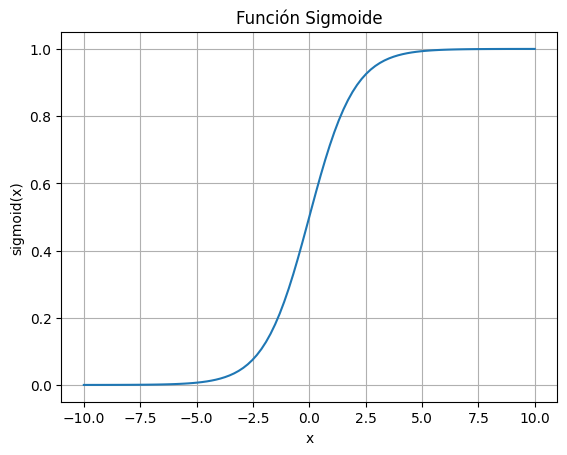
\includegraphics[width=.4\textwidth]{Imagenes/funcion_sigmoid.png}
    \caption{Gráfico de la ecuación de la función de activación sigmoide.}
    \label{fig:fun_sig}
\end{figure}

\textbf{Función Tanh}

La función de tangente hiperbólica conocida como función tanh, es una función suavizadora de centro cero cuyo rango se sitúa entre -1 y 1 como se muestra en la Figura \ref{fig:fun_tanh}, la salida de la función viene dada por la ecuación \ref{eq.tangentehip}. La función proporciona un rendimiento mayor en el entrenamiento de redes neuronales multicapa \citep{karlik2011performance, neal1992connectionist}. La principal ventaja de esta función es que produce una salida centrada en cero y es normalmente utilizada en redes neuronales recurrentes \citep{lecun2015deep}.

\begin{equation}
    \tanh(x) = \frac{e^x - e^{-x}}{e^x + e^{-x}}
    \label{eq.tangentehip}
\end{equation}

Sin embargo, esta función tanh no resuelve el problema de gradiente evanescente que sufren por igual las funciones sigmoidales y su propiedad de que solo puede alcanzar un gradiente de 1 cuando el valor de la entrada es 0, produce algunas neuronas muertas durante el cálculo, para resolver esta limitación existe la función de activación ReLU.

\begin{figure}[!h]
    \centering
    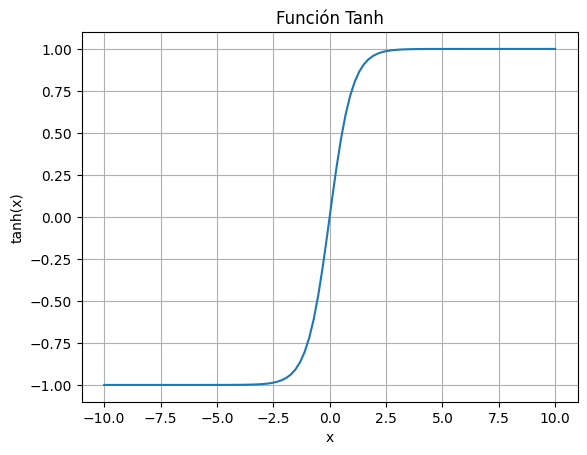
\includegraphics[width=.4\textwidth]{Imagenes/fun_tanh.png}
    \caption{Gráfico de la ecuación de la función de activación Tanh.}
    \label{fig:fun_tanh}
\end{figure}

\textbf{Función ReLU}

La función de unidad lineal rectificada (ReLU) ha sido la más frecuentemente utilizada para aplicaciones de aprendizaje profundo. La ReLU ofrece un mejor rendimiento y generalización en el aprendizaje profundo en comparación de la Sigmoide y Tanh. Su principal características es que representa a una función casi lineal y, por lo tanto, es más fácil de optimizar, con métodos de ascenso de gradiente \citep{nair2010rectified}.

La función ReLU realiza una operación de umbral a cada elemento de entrada donde los valores menores qué cero se ponen a cero y se representa con la siguiente ecuación \ref{eq.ReLU}.

\begin{equation}
    ReLU(x) = \max(0, x)
    \label{eq.ReLU}
\end{equation}

La funcion rectifica los valores de las entradas menores qué cero, forzándolos así a cero y eliminando el problema de gradiente evanescente como se muestra en la Figura \ref{fig:fun_relu}. Es normalmente utilizada en las capas ocultas y las capas de salida de la red, en tareas de clasificación de objetos \citep{krizhevsky2012imagenet}.

\begin{figure}[!h]
    \centering
    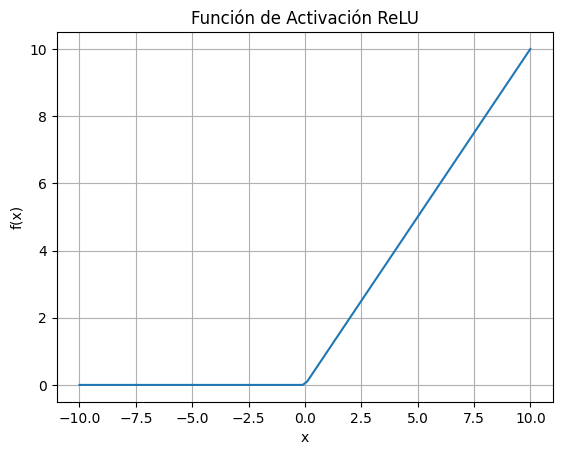
\includegraphics[width=.4\textwidth]{Imagenes/Fun_ReLU.png}
    \caption{Gráfico de la ecuación de la función de activación ReLU.}
    \label{fig:fun_relu}
\end{figure}

\textbf{Función Softmax}

La función Softmax se utiliza para calcular la distribución de probabilidades a partir de un vector de números reales. Esta produce una salida que es un rango entre 0 y 1, con la suma de las probabilidades igual a 1 (Figura \ref{fig:fun_softmax}), la función se muestra en la ecuación \ref{eq.Softmax}.

\begin{equation}
    \sigma(\mathbf{z})_i = \frac{e^{z_i}}{\sum_{j=1}^K e^{z_j}} \ \ \  \text{para } i = 1, ..., K
    \label{eq.Softmax}
\end{equation}

La función es utilizada en modelos de aprendizaje profundo enfocados en clasificación multiclase en los que se devuelve las probabilidades de cada clase y es normalmente usada en  las capas de salida \citep{krizhevsky2012imagenet}. La diferencia con la función sigmoide es que la softmax es para tareas de clasificación multivariante y la sigmoide en clasificación binaria.

\begin{figure}[!h]
    \centering
    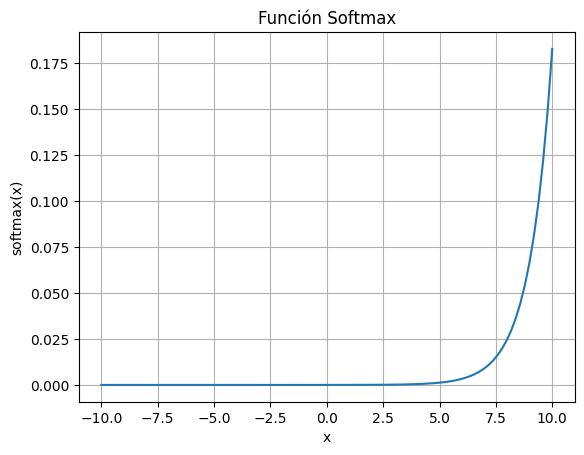
\includegraphics[width=.4\textwidth]{Imagenes/Func_softmax.png}
    \caption{Gráfico de la ecuación de la función de activación Softmax.}
    \label{fig:fun_softmax}
\end{figure}

\subsection{Inteligencia artificial}

La inteligencia artificial (IA) es un campo de la ciencia de la computación, que se enfoca en crear máquinas inteligentes que puedan razonar, aprender y actuar de manera autónoma \citep{rouhiainen2018inteligencia}.

Las tecnologías basadas en IA es usada para mejorar y disfrutar una mayor eficiencia en distintos ámbitos de la vida. La aplicación se puede realizar en diversas situaciones y algunas de las más importantes son las siguientes:

\begin{itemize}
    \item Reconocimiento de imágenes estáticas, clasificación y etiquetado.
    \item Mejoras del desempeño de la estrategia algorítmica comercial.
    \item Procesamiento eficiente y escalable de datos de pacientes.
    \item Mantenimiento predictivo.
    \item Detección y clasificación de objetos
    \item Protección contra amenazas de cibernética.
\end{itemize}

Dentro de la IA se encuentran diversas técnicas para crear sistemas inteligentes, como el aprendizaje automático y aprendizaje profundo que son subcampos que desempeñan un papel fundamental en el análisis de grandes cantidades de datos, identificar patrones y tendencias, de una forma más rápida y precisa (Figura~\ref{fig:IA_AA_A}).

  \begin{figure}[!h]
     \centering
     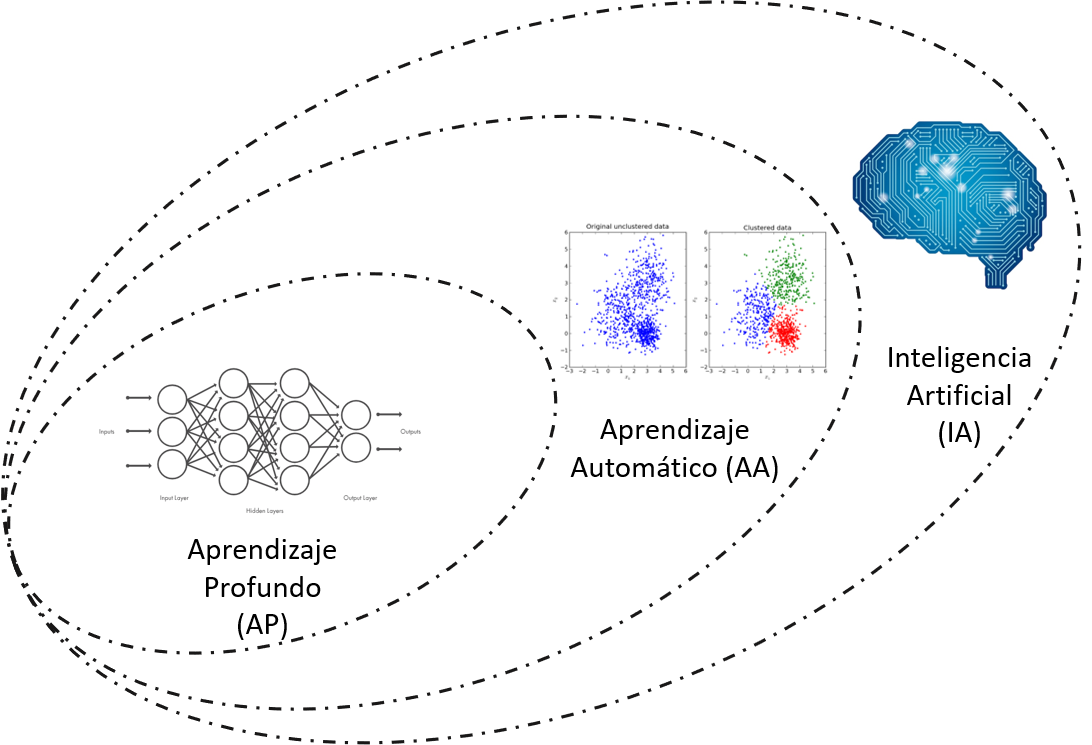
\includegraphics[width=.5\textwidth]{Imagenes/IA_AA_AP.png}
     \caption{Subcampos de la inteligencia artificial en el análisis de datos.}
     \label{fig:IA_AA_A}
 \end{figure}


\subsubsection{Aprendizaje Automático}

El aprendizaje automático (en inglés, \textit{machine learning}) se centra en el desarrollo de sistemas capaces de aprender de conjuntos de datos sin ser programados de manera explícita \citep{mitchell1997does}. Estos sistemas aprenden y mejoran su rendimiento en una tarea especifica a medida que se le presentan más datos. Un resultado típico serían las sugerencias o predicciones en una situación particular \citep{vieira2020main}.

Desde el punto de vista de ingeniería se define como un programa de computador que aprende de una experiencia E, con respecto a una tarea T y una medida de rendimiento R, si su rendimiento en T, medido por R, mejora con la experiencia E y también se puede definir como la ciencia de programar computadores para que aprendan a partir de un conjunto de datos \citep{geron2020aprende}.

\subsubsection{Aprendizaje Profundo}

El aprendizaje profundo (en inglés, \textit{deep learning}) es una rama del aprendizaje automático. A diferencia de los algoritmos tradicionales de aprendizaje automático, muchos de los cuales tienen una capacidad finita de aprendizaje independientemente de cuántos datos adquieran, los sistemas de aprendizaje profundo pueden mejorar su rendimiento al poder acceder a un mayor número de datos, o lo que es lo mismo, hacer que la máquina tenga más experiencia \citep{shinde2018review}. Una vez que las máquinas han conseguido suficiente experiencia mediante el aprendizaje profundo, pueden ponerse a trabajar para realizar tareas específicas como conducir un coche, detectar hierbajos en un campo de cultivo, detectar enfermedades, inspeccionar maquinaria para identificar errores, etc.

El aprendizaje profundo como se muestra en la Figura \ref{fig:AP} toma los fundamentos teóricos de las ANN clásicas, pero emplea una gran cantidad de neuronas y capas ocultas, junto con nuevos modelos y paradigmas de entrenamiento ofreciendo una capacidad mucho mayor para aprender a adaptarse y extraer características de datos de entrada de alta complejidad \citep{schmidhuber2015deep}. Las ANN usadas en el aprendizaje profundo son conocidas como redes neuronales profundas, en inglés \textit{Deep Neuronal Network} (DNN).

\begin{figure}[!h]
    \centering
    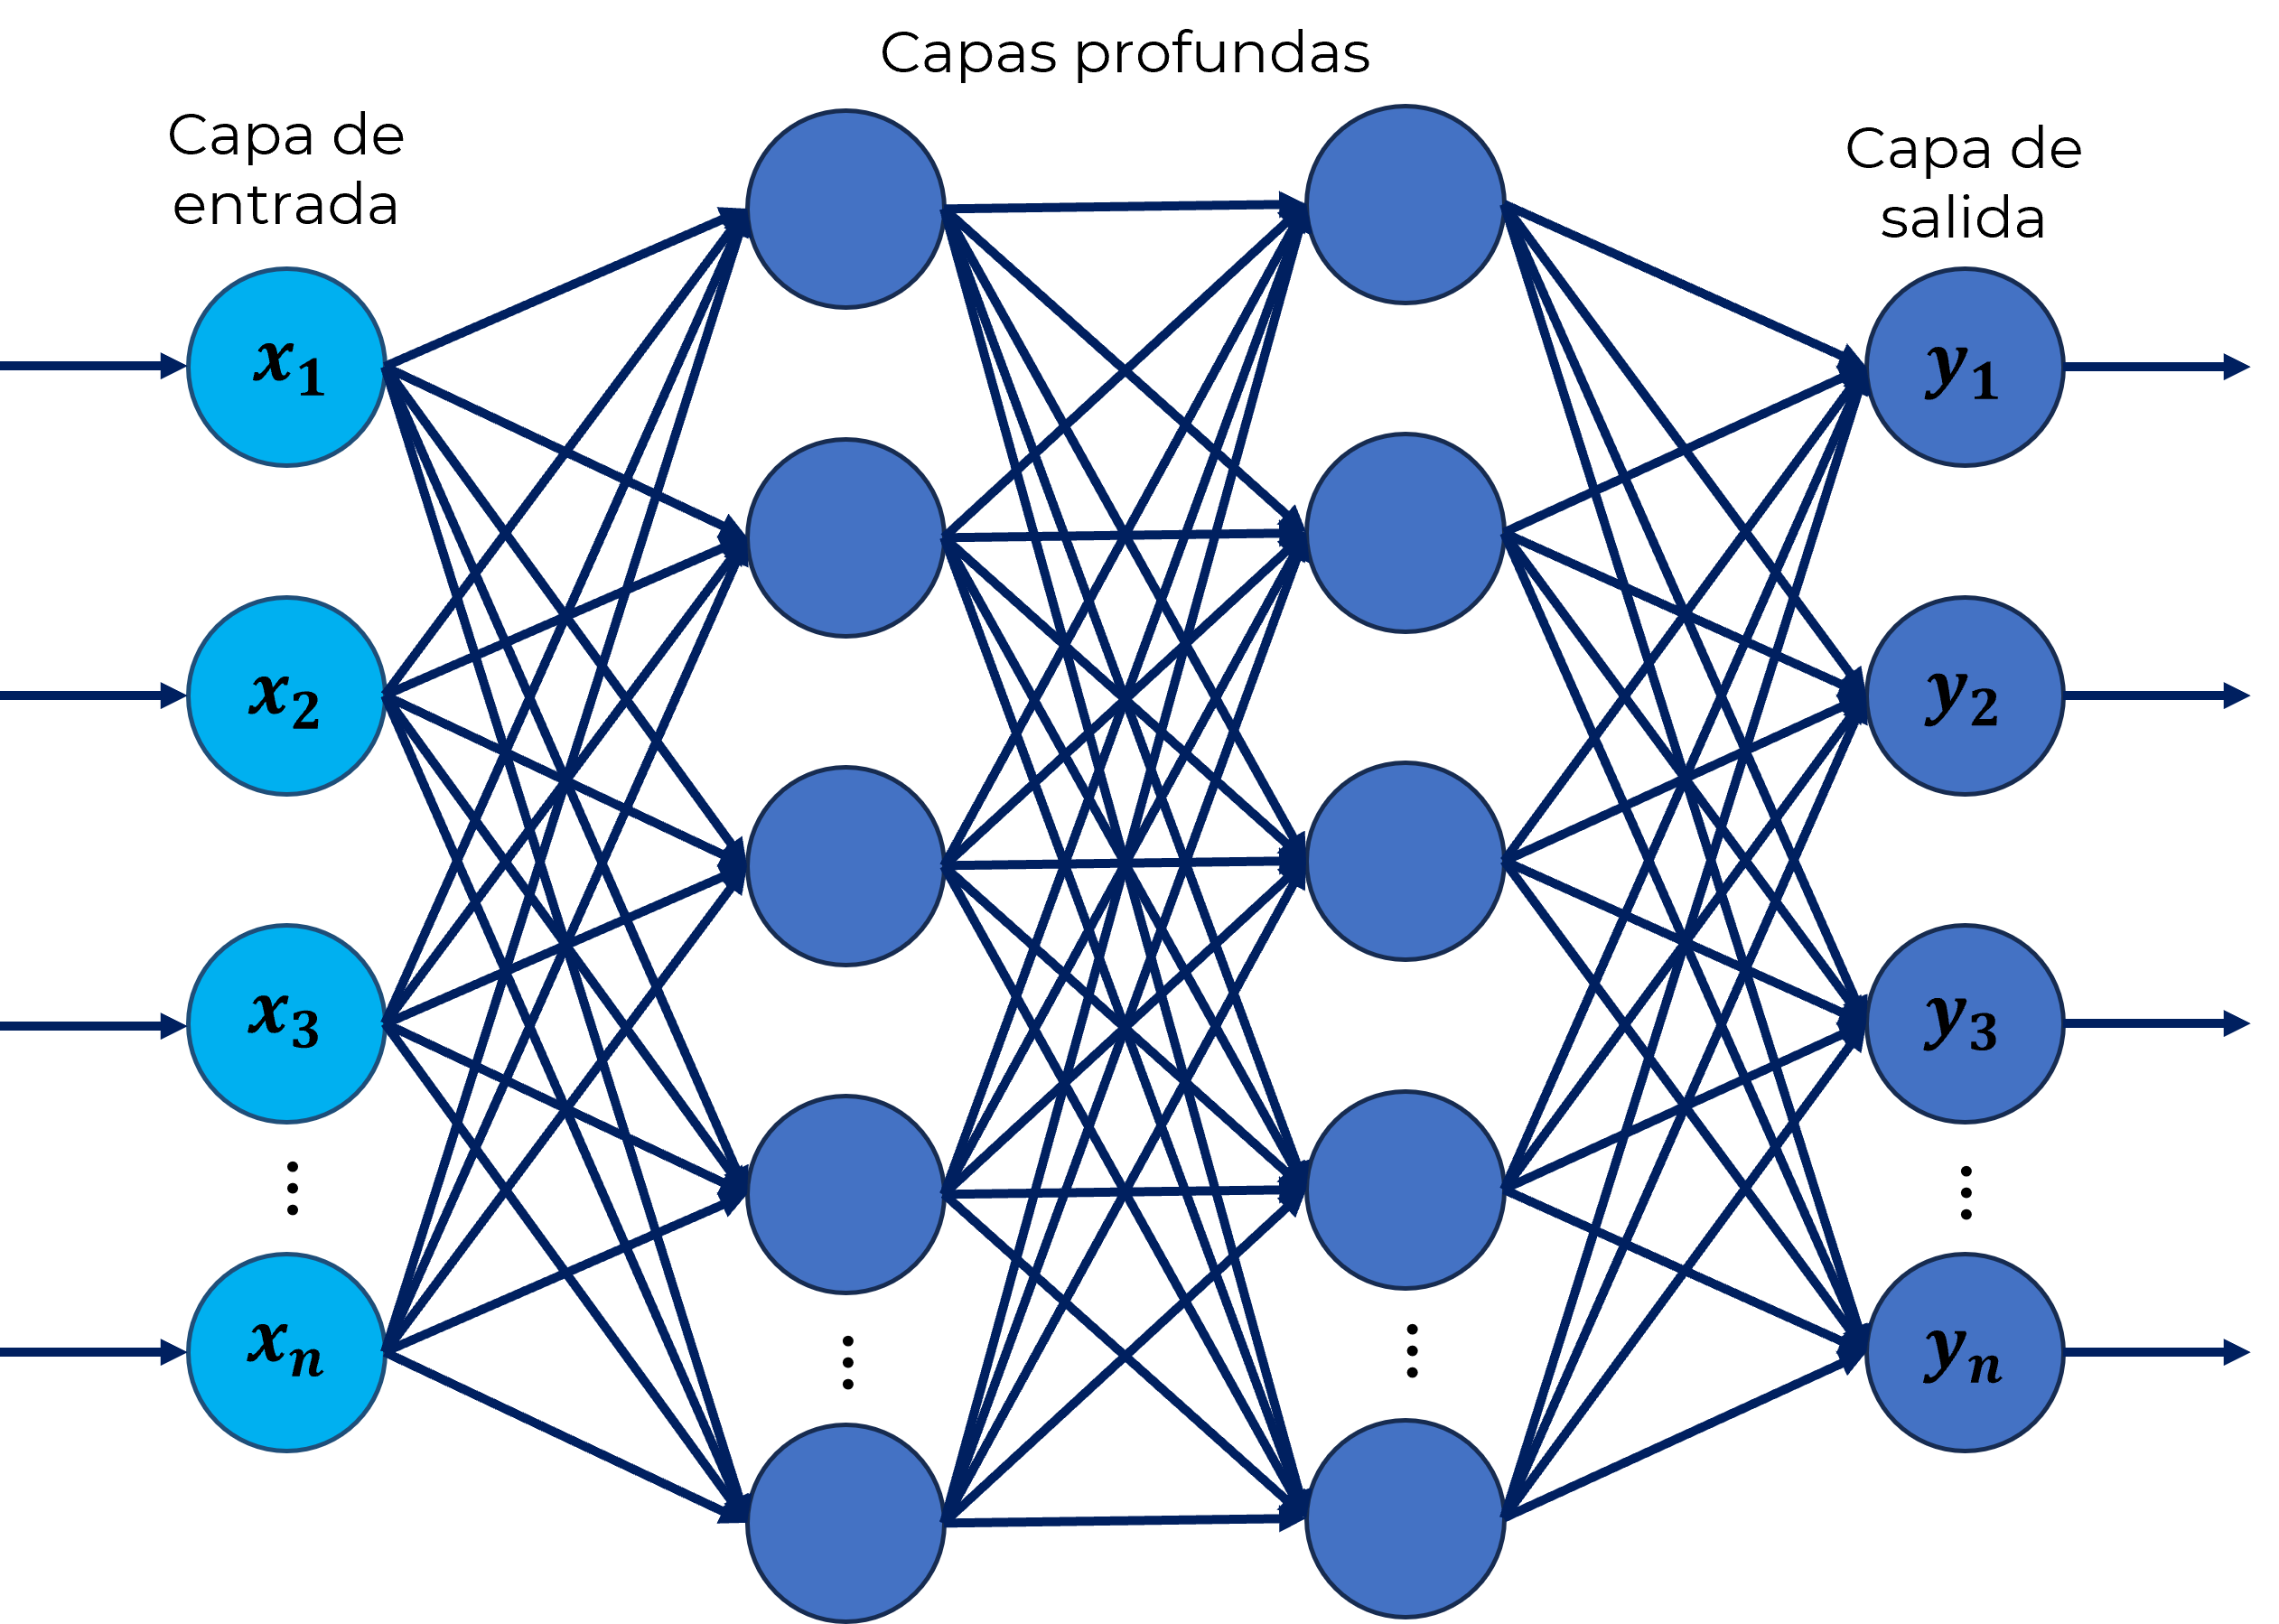
\includegraphics[width=.5\textwidth]{Imagenes/AP.png}
    \caption{Representación del aprendizaje profundo.}
    \label{fig:AP}
\end{figure}

\subsection{Red Neuronal Convolucional}

Las redes neuronales convolucionales, en inglés, \textit{Convolutional Neuronal Network} (CNN) son un tipo algoritmo propuesto por LeCun en 1989 \citep{lecun1989backpropagation}. La aplicación de las CNN se encuentra principalmente en el reconocimiento de voz, reconocimiento facial, reconocimiento de objetos, análisis de movimiento y procesamiento de lenguaje natural.

Las CNN habitualmente constan de múltiples capas de convolución acompañadas de capas de agrupación y una capa de neuronas completamente conectadas, como se muestra en la Figura~\ref{fig:CNN}.

  \begin{figure}[!h]
     \centering
     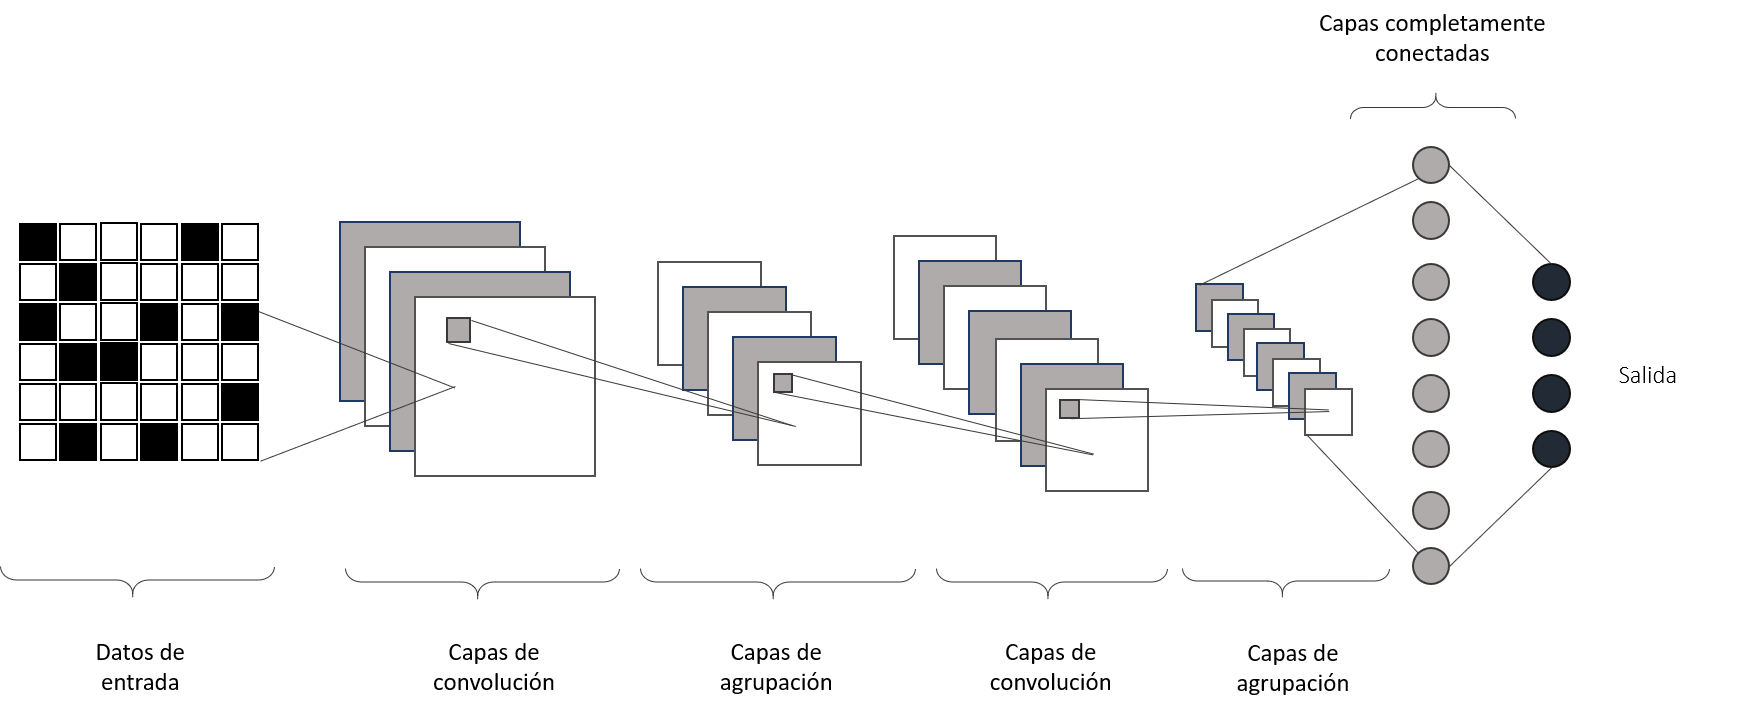
\includegraphics[width=.9\textwidth]{Imagenes/CNN.png}
     \caption{Diagrama de red convolucional simple.}
     \label{fig:CNN}
 \end{figure}

 La función de convolución se utiliza principalmente para extraer diversas características de los datos analizados. En proceso de la convolución cuenta de un núcleo de convolución, el cual se va deslizando en la ventana de entrada, de modo que los parámetros de peso en el núcleo se vayan multiplicando por los píxeles correspondientes. Posteriormente, los resultados siguen la multiplicación. En la Figura~\ref{fig:Convolution} se muestra el principio de la convolución.

 \begin{figure}[!h]
     \centering
     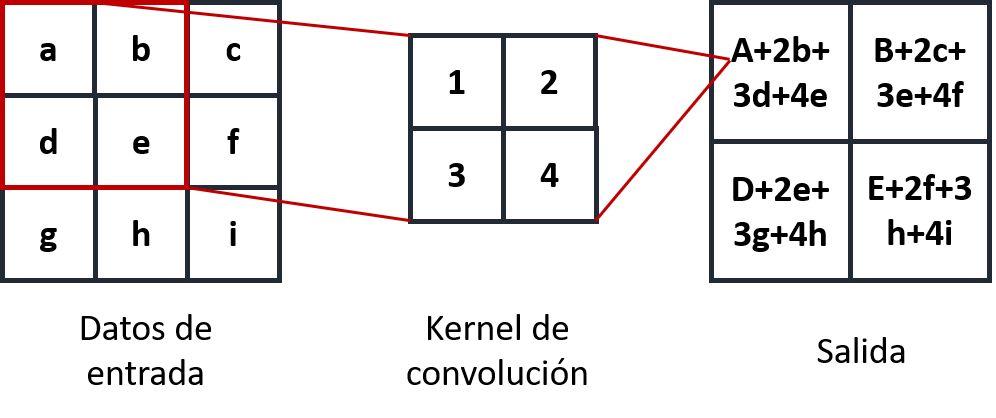
\includegraphics[width=.5\textwidth]{Imagenes/Convolucion.png}
     \caption{Diagrama esquemático de operación de convolución.}
     \label{fig:Convolution}
 \end{figure}

 La función de la capa de agrupación es abstraer la señal característica original, lo cual se realiza para reducir en gran medida los parámetros de entrenamiento y también poder reducir el grado de sobreajuste. Las operaciones de agrupación se dividen en dos categorías: agrupación máxima y agrupación media. En la agrupación máxima se toma el valor más grande de un pixel correspondiente como resultado del muestreo, y en la agrupación media se calcula el valor promedio del pixel correspondiente. En la Figura~\ref{fig:Agrupacion} se muestra el principio de la agrupación.

  \begin{figure}[!h]
     \centering
     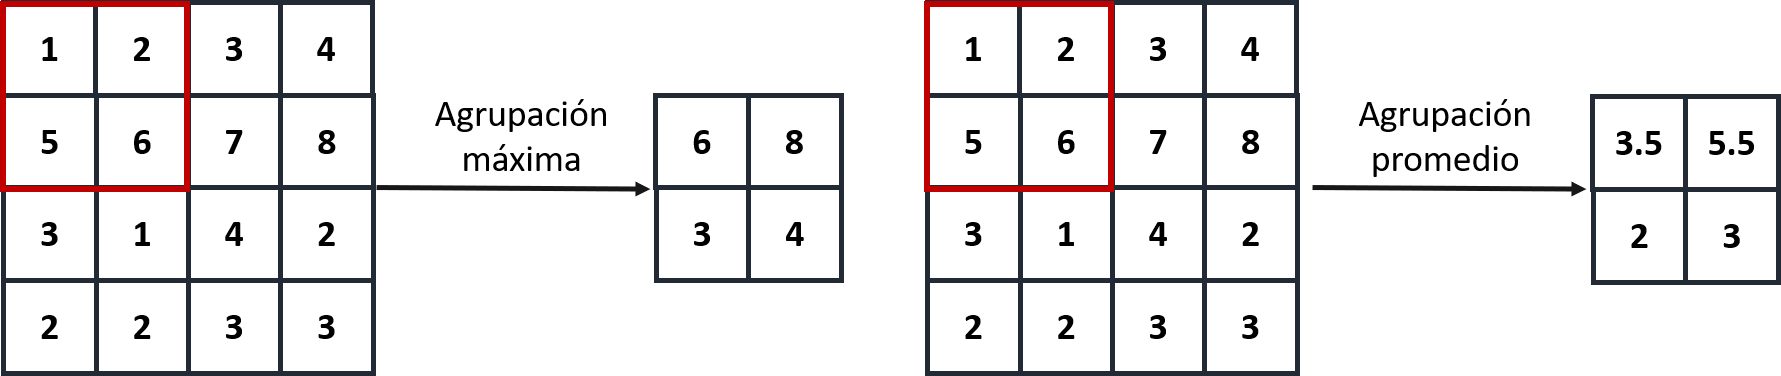
\includegraphics[width=.7\textwidth]{Imagenes/Agrupamiento.png}
     \caption{Diagrama esquemático de la operación de agrupación.}
     \label{fig:Agrupacion}
 \end{figure}

 \subsection{Red Neuronal Recurrente}

 Las redes neuronales recurrentes, en inglés, \textit{Recurrent Neuronal Network} (RNN) es un tipo de algoritmo propuesto en 1980. En los últimos años, las aplicaciones de las RNN han sido en muchos campos como: el procesamiento del lenguaje natural, el reconocimiento de imágenes y reconocimiento de voz.

 La característica principal de las RNN es que la entrada de la capa oculta incluye no solo la salida de capa de entrada, sino también la salida de la capa oculta en el último momento. Un modelo RNN simple puede ser expandido a una red compleja. En la Figura~\ref{fig:RNN} se puede observar la estructura de una RNN y el mapa de dependencia del orden temporal.

   \begin{figure}[!h]
     \centering
     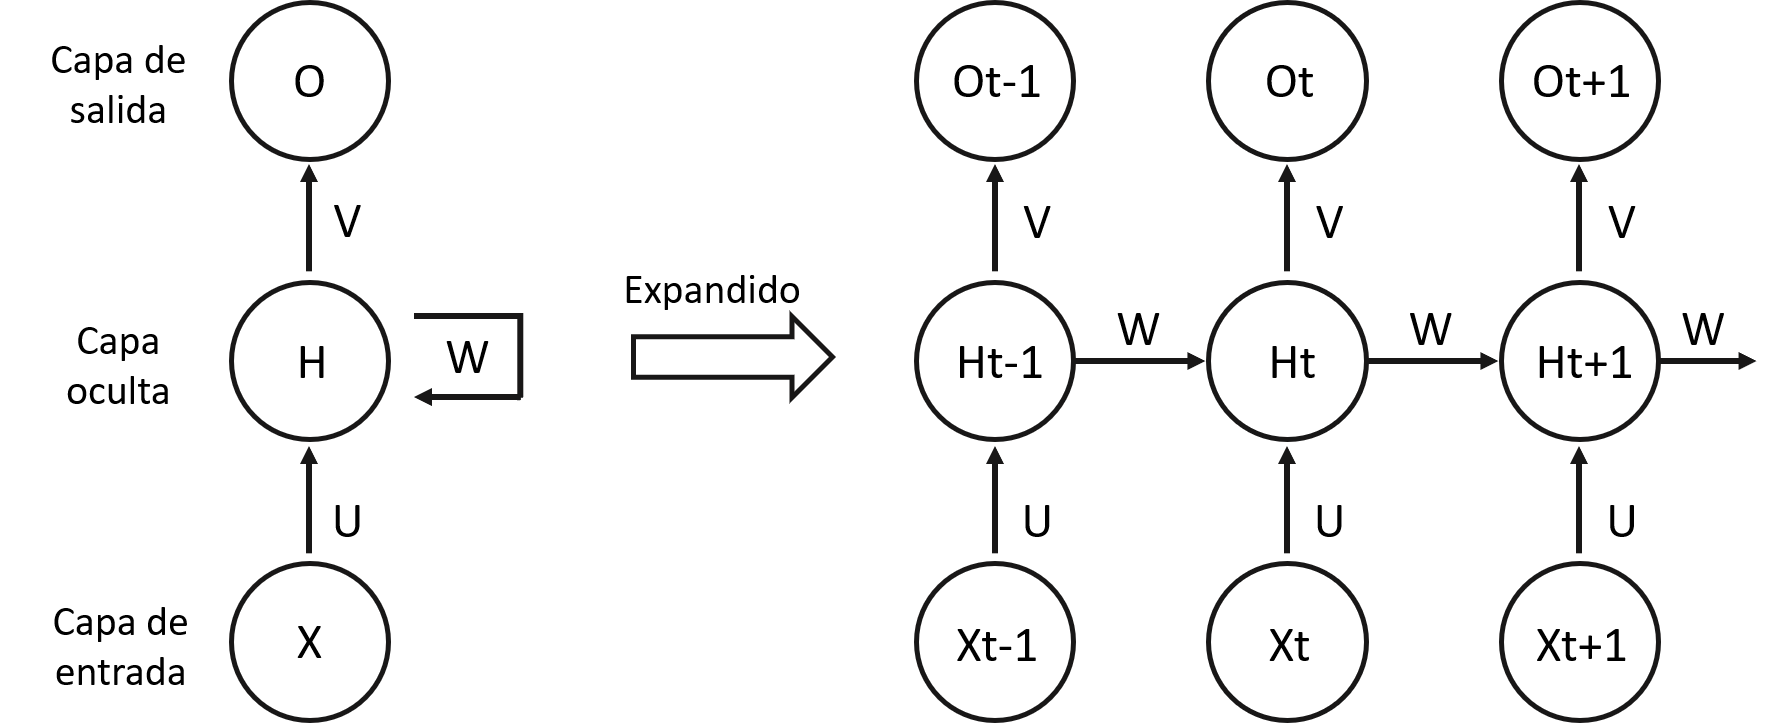
\includegraphics[width=.7\textwidth]{Imagenes/RNN.png}
     \caption{Estructura de la red neuronal recurrente simple y expandida.}
     \label{fig:RNN}
 \end{figure}

En la estructura de la RNN, Ht es el estado oculto del tiempo t y Ot representa la salida del tiempo t; U es el peso directo de la capa de entrada a la capa oculta; W es el peso de la capa oculta a la capa oculta, que es el controlador de memoria de la red que se encarga de programar la memoria; V es el peso de la capa oculta a la capa de salida, y las características aprendidas de la capa oculta pasaran a través de ella nuevamente y como salida final.

